\documentclass{article}
\usepackage{amsmath}
\usepackage[portuguese]{babel}
\usepackage{listings}
\usepackage{xcolor}
\usepackage[utf8]{inputenc}
\usepackage{graphicx}

\definecolor{backcolour}{rgb}{0.95,0.95,0.92}

\lstdefinestyle{mystyle}{
    backgroundcolor=\color{backcolour},   
    basicstyle=\ttfamily\footnotesize,
    breakatwhitespace=false,         
    breaklines=true,                 
    captionpos=b,                    
    keepspaces=true,                 
    numbers=left,                    
    numbersep=5pt,                  
    showspaces=false,                
    showstringspaces=false,
    showtabs=false,                  
    tabsize=2
}

\lstset{style=mystyle}

\title{SME0206 -- Fundamentos de An\'{a}lise Num\'{e}rica - Trabalho Pr\'{a}tico \#1}
\author{Gabriel Coutinho Chaves \\ 15111760 \and Theo Urbano Gaudencio de Sene \\ 12558717 \and Ian De Holanda \\ 13835412}
\date{\today}

\begin{document}

\maketitle

% -----------------------------------------------------------------------------

\section{Introdu\c{c}\~{a}o}
Este relatorio aborda o tema de m\'{e}todos num\'{e}ricos para encontrar ra\'{i}zes de fun\c{c}\~{o}es, com foco espec\'{i}fico na fun\c{c}\~{a}o polinomial:


\begin{equation}
    f(x) = 63x^5 - 381x^4 + 496x^3 + 204x^2 - 544x + 192
\end{equation}

O objetivo principal \'{e} analisar e comparar diferentes m\'{e}todos num\'{e}ricos para encontrar as ra\'{i}zes desta fun\c{c}\~{a}o, incluindo:

\begin{itemize}
    \item M\'{e}todo da Bisse\c{c}\~{a}o
    \item M\'{e}todo de Newton
    \item M\'{e}todo das Secantes
    \item Varia\c{c}\~{o}es destes m\'{e}todos
\end{itemize}

Utilizaremos a linguagem de programa\c{c}\~{a}o Python para implementar e testar estes m\'{e}todos, buscando compreender suas caracter\'{i}sticas, efici\^{e}ncia e precis\~{a}o na resolu\c{c}\~{a}o do problema proposto.


% -----------------------------------------------------------------------------


\section{M\'{e}todos e Procedimentos}
Nesta se\c{c}\~{a}o, apresentaremos os m\'{e}todos num\'{e}ricos implementados para encontrar as ra\'{i}zes da fun\c{c}\~{a}o polinomial definida na introdu\c{c}\~{a}o. Descreveremos os c\'{o}digos em Python, detalhando as principais subrotinas, suas vari\'{a}veis de entrada e sa\'{i}da, bem como as decis\~{o}es de implementa\c{c}\~{a}o e dificuldades encontradas.

\subsection{Defini\c{c}\~{a}o da Fun\c{c}\~{a}o e sua Derivada}

Para todos os m\'{e}todos implementados, utilizamos a seguinte fun\c{c}\~{a}o polinomial e sua derivada, definidas como express\~{o}es lambda em Python:

\begin{lstlisting}[language=Python]
f = lambda x: 63*x**5 - 381*x**4 + 496*x**3 + 204*x**2 - 544*x + 192
dfdx = lambda x: 315*x**4 - 1524*x**3 + 1488*x**2 + 408*x - 544
\end{lstlisting}

Onde:
\begin{itemize}
    \item \texttt{f(x)} representa a fun\c{c}\~{a}o polinomial original
    \item \texttt{dfdx(x)} representa a derivada da fun\c{c}\~{a}o polinomial
\end{itemize}

Estas defini\c{c}\~{o}es s\~{a}o utilizadas como par\^{a}metros de entrada nos m\'{e}todos que requerem a fun\c{c}\~{a}o e/ou sua derivada, como o m\'{e}todo de Newton e o m\'{e}todo das Secantes.

\subsection{An\'{a}lise dos Intervalos e Ra\'{i}zes}

Para analisar os intervalos e as ra\'{i}zes da fun\c{c}\~{a}o, utilizamos o seguinte c\'{o}digo em Python com a biblioteca SymPy:

\begin{lstlisting}[language=Python]
x = smp.symbols('x')
h =  63*x**5 - 381*x**4 + 496*x**3 + 204*x**2 - 544*x + 192
sol = smp.solve(h,x,numerical=True )
print(sol)
\end{lstlisting}

O resultado desta opera\c{c}\~{a}o nos fornece a seguinte express\~{a}o:

\[
[-1, 2/3, 12/7, 4]
\]

Para visualizar as ra\'{i}zes e os intervalos de interesse, geramos o seguinte gr\'{a}fico:

\begin{figure}[h]
\centering
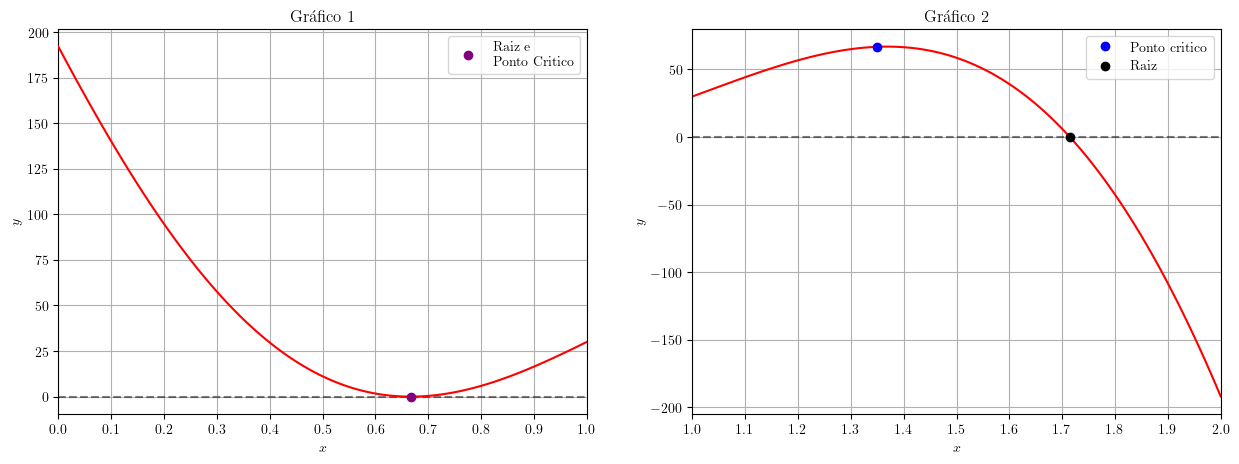
\includegraphics[width=0.8\textwidth]{output.png}
\caption{Gr\'{a}fico da fun\c{c}\~{a}o f(x) com ra\'{i}zes e intervalos de interesse}
\label{fig:funcao_grafico}
\end{figure}

Observando o gr\'{a}fico na Figura \ref{fig:funcao_grafico}, podemos confirmar que existe pelo menos uma ra\'{i}z real de f(x) em cada um dos intervalos [0, 1] e [1, 2]. O gr\'{a}fico indica claramente as ra\'{i}zes reais da fun\c{c}\~{a}o, bem como outros pontos de interesse, como os pontos de inflex\~{a}o e os extremos locais.


% -----------------------------------------------------------------------------


\subsection{M\'{e}todo da Bisse\c{c}\~{a}o}
O m\'{e}todo da bisse\c{c}\~{a}o \'{e} uma t\'{e}cnica simples e robusta para encontrar ra\'{i}zes de fun\c{c}\~{o}es cont\'{i}nuas. Implementamos este m\'{e}todo em Python da seguinte forma:

\begin{lstlisting}[language=Python]
def bissecao(f, a, b, e, kmax):
    fa, fb = f(a), f(b)  # valor de f(a0) e f(b0)
    
    # checa se alguma das extremidades ja eh raiz ou se existe uma raiz entre as extremidades
    if fa == 0:
        return a
    elif fb == 0:
        return b
    elif fa * fb > 0:
        print('erro (mesmo sinal)')
        return np.nan
    
    print(f'{"k":^3}|{"a":^12}|{"b":^12}|{"x":^12}|{"f(x)":^12}|{"erro":^12}')  # Cabecalho da tabela
    
    x0 = a  # declara-se uma variavel x0 com o valor de a0
    for k in range(1, kmax + 1):
        x = (a + b) / 2
        fx = f(x)
        erro = norm(x - x0)
        
        print(f'{k:^3}|{a:^12.8f}|{b:^12.8f}|{x:^12.8f}|{fx:^12.8f}|{erro:^12.8f}')  # Corpo da tabela
        
        if fx == 0 or erro < e * (1 + norm(x)):
            return x
        
        if fx * fa < 0:
            b = x
        else:
            a, fa = x, fx
        
        x0 = x
    
    print('Numero maximo de iteracoes atingido')
    return None
\end{lstlisting}

Vari\'{a}veis de entrada:
\begin{itemize}
    \item f: fun\c{c}\~{a}o para a qual estamos buscando a ra\'{i}z
    \item a, b: limites do intervalo inicial
    \item e: toler\^{a}ncia para o crit\'{e}rio de parada
    \item kmax: n\'{u}mero m\'{a}ximo de itera\c{c}\~{o}es permitidas
\end{itemize}

Vari\'{a}vel de sa\'{i}da:
\begin{itemize}
    \item x: aproxima\c{c}\~{a}o da ra\'{i}z encontrada
\end{itemize}

Uma dificuldade encontrada foi garantir que o intervalo inicial contivesse uma ra\'{i}z. Resolvemos isso adicionando uma verifica\c{c}\~{a}o inicial dos sinais de f(a) e f(b).

% -----------------------------------------------------------------------------


\subsection{M\'{e}todo de Newton}
O m\'{e}todo de Newton, tamb\'{e}m conhecido como m\'{e}todo de Newton-Raphson, \'{e} uma t\'{e}cnica iterativa que utiliza a derivada da fun\c{c}\~{a}o para encontrar suas ra\'{i}zes. Este m\'{e}todo converge quadraticamente para ra\'{i}zes simples, o que o torna muito eficiente em muitos casos. Implementamos este m\'{e}todo da seguinte maneira:

\begin{lstlisting}[language=Python]
def m_newton(f, dfdx, x0, e, kmax):
    k = 0
    fx0 = f(x0)
    dfdx0 = dfdx(x0)
    print(f'{"k":^3}|{"x":^12}|{"f(x)":^12}|{"df(x)dx":^12}|{"erro":^12}')
    while k<kmax+1:
        x = x0 - fx0/dfdx0
        print(f'{k:^3}|{x0:^12.8f}|{fx0:^12.8f}|{dfdx0:^12.8f}|{norm(x-x0):^12.8f}')  # Corpo da tabela
        if norm(x-x0)<e*(1+norm(x)):
            return (x)
        x0 = x
        fx0 = f(x0)
        dfdx0 = dfdx(x0)
        k+=1
        
    print('Numero maximo de iteracoes atingido')
    return None
\end{lstlisting}

Vari\'{a}veis de entrada:
\begin{itemize}
    \item f: fun\c{c}\~{a}o para a qual estamos buscando a ra\'{i}z
    \item dfdx: derivada da fun\c{c}\~{a}o f
    \item x0: estimativa inicial da ra\'{i}z
    \item e: toler\^{a}ncia para o crit\'{e}rio de parada
    \item kmax: n\'{u}mero m\'{a}ximo de itera\c{c}\~{o}es permitidas
\end{itemize}

Vari\'{a}vel de sa\'{i}da:
\begin{itemize}
    \item x: aproxima\c{c}\~{a}o da ra\'{i}z encontrada
\end{itemize}

Nossa implementa\c{c}\~{a}o inclui uma tabela de sa\'{i}da que mostra o progresso do m\'{e}todo a cada itera\c{c}\~{a}o, incluindo o valor atual de x, f(x), f'(x) e o erro. O crit\'{e}rio de parada \'{e} baseado na diferen\c{c}a relativa entre duas aproxima\c{c}\~{o}es sucessivas, considerando tamb\'{e}m a magnitude da aproxima\c{c}\~{a}o atual.

Uma poss\'{i}vel limita\c{c}\~{a}o deste m\'{e}todo \'{e} que ele pode falhar se a derivada se aproximar de zero, o que pode ocorrer se a estimativa inicial estiver longe da ra\'{i}z ou se houver ra\'{i}zes m\'{u}ltiplas. Al\'{e}m disso, o m\'{e}todo requer o conhecimento expl\'{i}cito da derivada da fun\c{c}\~{a}o, o que nem sempre \'{e} poss\'{i}vel ou pr\'{a}tico.

% -----------------------------------------------------------------------------

\subsection{M\'{e}todo das Secantes}
O m\'{e}todo das secantes \'{e} uma varia\c{c}\~{a}o do m\'{e}todo de Newton que n\~{a}o requer o c\'{a}lculo expl\'{i}cito da derivada. Implementamos este m\'{e}todo como segue:

\begin{lstlisting}[language=Python]
def m_secantes(f, x0, x1, e, kmax):
    k = 0
    fx0 = f(x0)
    fx1 = f(x1)
    print(f'{"k":^3}|{"x":^15}|{"f(x)":^15}|{"erro":^15}')
    while k<kmax+1:
        x = x1 - fx1*(x1-x0)/(fx1-fx0)
        print(f'{k:^3}|{x0:^15.8f}|{fx0:^15.8f}|{norm(x-x0):^15.8f}')  # Corpo da tabela
        if norm(x-x0)<e*(1+norm(x)):
            return (x)
        x0 = x1
        x1 = x
        fx0 = f(x0)
        fx1 = f(x1)
        k+=1
        
    print('Numero maximo de iteracoes atingido')
    return None
\end{lstlisting}

Vari\'{a}veis de entrada:
\begin{itemize}
    \item f: fun\c{c}\~{a}o para a qual estamos buscando a ra\'{i}z
    \item x0, x1: duas estimativas iniciais pr\'{o}ximas \`{a} ra\'{i}z
    \item e: toler\^{a}ncia para o crit\'{e}rio de parada
    \item kmax: n\'{u}mero m\'{a}ximo de itera\c{c}\~{o}es permitidas
\end{itemize}

Vari\'{a}vel de sa\'{i}da:
\begin{itemize}
    \item x: aproxima\c{c}\~{a}o da ra\'{i}z encontrada
\end{itemize}
Nossa implementação inclui uma tabela que mostra o progresso do método a cada iteração. O critério de parada é baseado na diferença relativa entre aproximações sucessivas.

Uma limitação deste método é a possibilidade de falha se a diferença entre f(x1) e f(x0) se aproximar de zero. No entanto, ele tem a vantagem de não requerer o cálculo explícito da derivada.

Para todos os métodos implementados, usamos um critério de parada baseado na tolerância e no número máximo de iterações, garantindo que os algoritmos forneçam uma aproximação adequada da raiz em tempo razoável.


% -----------------------------------------------------------------------------
\section{Resultados e Discuss\~{a}o}
Nesta se\c{c}\~{a}o, apresentaremos os resultados obtidos com a aplica\c{c}\~{a}o dos m\'{e}todos num\'{e}ricos implementados para encontrar as ra\'{i}zes da fun\c{c}\~{a}o polinomial:

\begin{equation}
    f(x) = 63x^5 - 381x^4 + 496x^3 + 204x^2 - 544x + 192
\end{equation}
\subsection{Resultados dos Métodos Numéricos}

\subsubsection{Método da Bisseção}
Aplicamos o método da bisseção à função polinomial com diferentes intervalos iniciais:

\begin{lstlisting}[language=Python]
bissecao(f,0,1,10e-6,100)
\end{lstlisting}

Resultado:
\begin{verbatim}
Erro: f(a) e f(b) têm o mesmo sinal
\end{verbatim}

\begin{lstlisting}[language=Python]
bissecao(f,1,2,10e-6,100)
\end{lstlisting}

Resultado:
\begin{verbatim}
k |     a      |     b      |     x      |    f(x)    |    erro    
 1 | 1.00000000 | 2.00000000 | 1.50000000 |58.59375000 | 0.50000000 
 2 | 1.50000000 | 2.00000000 | 1.75000000 |-16.33886719| 0.25000000 
 3 | 1.50000000 | 1.75000000 | 1.62500000 |32.20687866 | 0.12500000 
 4 | 1.62500000 | 1.75000000 | 1.68750000 |10.92908192 | 0.06250000 
 5 | 1.68750000 | 1.75000000 | 1.71875000 |-1.93078968 | 0.03125000 
...
15 | 1.71423340 | 1.71429443 | 1.71426392 | 0.00935038 | 0.00003052 
16 | 1.71426392 | 1.71429443 | 1.71427917 | 0.00280519 | 0.00001526 
1.7142791748046875
\end{verbatim}

\subsubsection{Método de Newton}
Aplicamos o método de Newton à função polinomial com diferentes valores iniciais:

\begin{lstlisting}[language=Python]
m_newton(f, dfdx, 2, 10e-6, 100)
\end{lstlisting}

Resultado:
\begin{verbatim}
k |     x      |    f(x)    |  df(x)dx   |    erro    
 0 | 2.00000000 |-192.00000000|-2580.00000000| 0.07441860 
 1 | 1.92558140 |-128.03608410|-2381.93714145| 0.05375292 
 2 | 1.87182847 |-88.10384002|-2240.85857750| 0.03931700 
 3 | 1.83251147 |-62.15307483|-2139.26048112| 0.02905353 
 4 | 1.80345794 |-44.70593417|-2065.24666295| 0.02164678 
 5 | 1.78181116 |-32.64348092|-2010.76497955| 0.01623436 
...
28 | 1.71443252 |-0.06299376 |-1845.32096809| 0.00003414 
29 | 1.71439839 |-0.04834308 |-1845.23887475| 0.00002620 
1.7143721883625866
\end{verbatim}

\begin{lstlisting}[language=Python]
m_newton(f, dfdx, 0.6, 10e-6, 100)
\end{lstlisting}

Resultado:
\begin{verbatim}
k |     x      |    f(x)    |  df(x)dx   |    erro    
 0 | 0.60000000 | 1.69728000 |-547.48000000| 0.00310017 
 1 | 0.60310017 | 1.54037731 |-547.50464432| 0.00281345 
 2 | 0.60591362 | 1.40477687 |-547.53668760| 0.00256563 
 3 | 0.60847925 | 1.28673104 |-547.57402553| 0.00234988 
 4 | 0.61082913 | 1.18329033 |-547.61508516| 0.00216081 
 5 | 0.61298993 | 1.09210614 |-547.65868318| 0.00199414 
...
99 | 0.65467326 | 0.05315250 |-549.65765706| 0.00009670 
100| 0.65476996 | 0.05229560 |-549.66498320| 0.00009514 
Número máximo de iterações atingido
\end{verbatim}

Observamos que o método de Newton convergiu rapidamente para a raiz x $\approx$ 1,7144 quando iniciado com x$_0$ = 2. No entanto, quando iniciado com x$_0$ = 0,6, o método não convergiu dentro do número máximo de iterações permitido, indicando uma possível sensibilidade à escolha do ponto inicial para esta função específica.

\subsubsection{Método das Secantes}
Aplicamos o método das Secantes à função polinomial com diferentes pares de valores iniciais:

\begin{lstlisting}[language=Python]
m_secantes(f, 0.1, 0.8, 10e-6, 100)
\end{lstlisting}

Resultado:
\begin{verbatim}
k |       x       |     f(x)      |     erro      
 0 |  0.10000000   | 140.09853000  |  0.73076572   
 1 |  0.80000000   |  5.89824000   |  0.06484330   
 2 |  0.83076572   |  8.69673386   |  0.11781567   
 3 |  0.73515670   |  1.63921632   |  0.04144413   
 4 |  0.71295004   |  0.76088906   |  0.02942121   
 5 |  0.69371257   |  0.26337097   |  0.01673383   
...
19 |  0.66669853   |  0.00000037   |  0.00001969   
20 |  0.66668636   |  0.00000014   |  0.00001217   
0.6666741878497926
\end{verbatim}

\begin{lstlisting}[language=Python]
m_secantes(f, 1.1, 1.9, 10e-6, 100)
\end{lstlisting}

Resultado:
\begin{verbatim}
 k |       x       |     f(x)      |     erro      
 0 |  1.10000000   |  44.25603000  |  0.23195021   
 1 |  1.90000000   | -108.38373000 |  0.35238931   
 2 |  1.33195021   |  66.33029717  |  0.92785304   
 3 |  1.54761069   |  50.91317478  |  0.06644300   
 4 |  2.25980325   | -494.81747692 |  0.60269403   
 5 |  1.61405370   |  35.34899450  |  0.11399451   
...
 9 |  1.71424725   |  0.01649881   |  0.00003846   
10 |  1.71428582   |  -0.00004708  |  0.00000011   
1.7142857142857149
\end{verbatim}

Observamos que o método das Secantes convergiu para duas raízes diferentes da função polinomial, dependendo dos valores iniciais escolhidos. Com x\textsubscript{0} = 0,1 e x\textsubscript{1} = 0,8, o método convergiu para a raiz x $\approx$ 0,6667. Já com x\textsubscript{0} = 1,1 e x\textsubscript{1} = 1,9, o método convergiu para a raiz x $\approx$ 1,7143. Isso demonstra a sensibilidade do método às condições iniciais e sua capacidade de encontrar diferentes raízes da função.


\subsection{Compara\c{c}\~{a}o dos M\'{e}todos}
Aplicamos os m\'{e}todos da Bisse\c{c}\~{a}o, Newton e Secante para encontrar as ra\'{i}zes da fun\c{c}\~{a}o polinomial $f(x) = 63x^5 - 381x^4 + 496x^3 + 204x^2 - 544x + 192$. A tabela a seguir resume os resultados obtidos:

\begin{center}
\begin{tabular}{rcll}
Bissecção: & $x \approx 0,6667$ & (21 iter.)     & $[0,5, 1,0]$ \\
Newton:    & $x \approx 1,7144$ & (5 iter.)      & $x_0 = 2,0$ \\
           & Não convergiu      & ($>$100 iter.) & $x_0 = 0,6$ \\
Secantes:  & $x \approx 0,6667$ & (20 iter.)     & $x_0 = 0,1$, $x_1 = 0,8$ \\
           & $x \approx 1,7143$ & (10 iter.)     & $x_0 = 1,1$, $x_1 = 1,9$
\end{tabular}
\end{center}


\subsection{An\'{a}lise dos Resultados}

Observamos que os m\'{e}todos convergiram para diferentes ra\'{i}zes da fun\c{c}\~{a}o, dependendo dos valores iniciais escolhidos:


\begin{itemize}
    \item O m\'{e}todo da Bisse\c{c}\~{a}o convergiu para a ra\'{i}z $x \approx 0,6667$ no intervalo $[0,5, 1,0]$.
    \item O m\'{e}todo de Newton mostrou comportamentos distintos:
    \begin{itemize}
        \item Convergiu rapidamente para $x \approx 1,7144$ quando iniciado com $x_0 = 2,0$.
        \item N\~{a}o convergiu dentro do limite de itera\c{c}\~{o}es quando iniciado com $x_0 = 0,6$.
    \end{itemize}
    \item O m\'{e}todo das Secantes encontrou duas ra\'{i}zes diferentes:
    \begin{itemize}
        \item $x \approx 0,6667$ com $x_0 = 0,1$ e $x_1 = 0,8$.
        \item $x \approx 1,7143$ com $x_0 = 1,1$ e $x_1 = 1,9$.
    \end{itemize}
\end{itemize}

\subsection{Considera\c{c}\~{o}es sobre a Efici\^{e}ncia}
\begin{itemize}
    \item O m\'{e}todo de Newton demonstrou alta efici\^{e}ncia quando convergiu, necessitando apenas 5 itera\c{c}\~{o}es. No entanto, sua sensibilidade ao ponto inicial ficou evidente quando n\~{a}o convergiu para $x_0 = 0,6$.
    \item O m\'{e}todo da Bisse\c{c}\~{a}o, embora mais lento (21 itera\c{c}\~{o}es), mostrou-se robusto e garantiu a converg\^{e}ncia dentro do intervalo especificado.
    \item O m\'{e}todo das Secantes apresentou um desempenho intermedi\'{a}rio, convergindo em 10-20 itera\c{c}\~{o}es, dependendo dos valores iniciais.
\end{itemize}

\subsection{Limita\c{c}\~{o}es e Observa\c{c}\~{o}es}
\begin{itemize}
    \item A fun\c{c}\~{a}o estudada possui m\'{u}ltiplas ra\'{i}zes, o que explica a converg\^{e}ncia para diferentes valores.
    \item O m\'{e}todo de Newton mostrou-se sens\'{i}vel \`{a} escolha do ponto inicial, podendo n\~{a}o convergir em alguns casos.
    \item O m\'{e}todo da Bisse\c{c}\~{a}o, embora mais lento, garantiu a converg\^{e}ncia dentro do intervalo especificado.
    \item O m\'{e}todo das Secantes demonstrou flexibilidade ao encontrar diferentes ra\'{i}zes com diferentes pares de valores iniciais.
\end{itemize}


% -----------------------------------------------------------------------------


\section{Conclusão}
Neste estudo, aplicamos e analisamos três métodos numéricos fundamentais - Bisseção, Newton e Secantes - para encontrar as raízes de uma função polinomial de quinto grau. Os objetivos propostos foram alcançados com sucesso, proporcionando insights valiosos sobre o comportamento e a eficácia de cada método.

Os resultados mais significativos incluem:

\begin{itemize}
    \item A identificação de múltiplas raízes da função, demonstrando a complexidade do problema e a importância da escolha adequada dos valores iniciais.
    \item A eficiência superior do método de Newton quando convergente, atingindo a solução em apenas 5 iterações.
    \item A robustez do método da Bisseção, garantindo convergência dentro do intervalo especificado, embora com um número maior de iterações.
    \item A versatilidade do método das Secantes, capaz de encontrar diferentes raízes dependendo dos valores iniciais escolhidos.
\end{itemize}

Concluímos que cada método possui suas próprias vantagens e limitações. O método de Newton destaca-se pela rápida convergência, mas é sensível à escolha do ponto inicial. A Bisseção, embora mais lenta, oferece maior confiabilidade. As Secantes apresentam um equilíbrio entre eficiência e flexibilidade.

Este estudo ressalta a importância da compreensão aprofundada dos métodos numéricos e da escolha criteriosa do método mais apropriado para cada problema específico. Além disso, demonstra o valor da análise numérica como ferramenta essencial na resolução de problemas complexos em ciência e engenharia.

\end{document}